\section{Introduzione}

L'iterazione 1 ha come scopo quello di identificare le componenti dal modello dei casi d'uso, 
applicando le euristiche di early design: verrà perfezionata la specifica dei componenti 
progettati durante l'iterazione 0 al fine di da definire meglio l'architettura software. 
È stato costruito lo scheletro dell'applicazione tramite la specifica delle differenti classi 
popolate nelle seguenti iterazioni.

Inizialmente, durante lo sviluppo dell'iterazione 0, il sistema nella sua totalità è stato 
visualizzato come una unica componente e sono stati 
introdotti gli attori, ognuno dei quali definito come un'entità esterna. In seguito sono stati 
sviluppati tutti i casi d'uso che riassumono il funzionamento del sistema, i quali verranno, 
nell'Iterazione 1, raccolti e raggruppati secondo un preciso criterio e affinità. 

Vengono inoltre introdotti componenti e sottocomponenti di controllo di ciascun gruppo, o 
alternativamente componenti di dati; per ognuna di esse nascono parallelamente le classi 
candidate e le relazioni che le legano. 

Per ogni caso d'uso che ha una interazione diretta con un attore esterno viene introdotta 
un'interfaccia per le operazioni visibili esternamente, ovvero le API, offerte o richieste 
dal componente o sottocomponente corrispondente, in base alla direzione dell'interazione. 

Ogni variabile input da un attore, specificata nella descrizione di un caso d'uso, 
definisce un parametro di input dell'operazione dell'interfaccia corrispondente. 
Ogni variabile output per un attore specificata nella descrizione di un caso d'uso 
definisce un parametro di ritorno dell'operazione dell'interfaccia corrispondente 
(se modalità sincrona) o un input di un'operazione dell'interfaccia di callback (se modalità asincrona) dell'attore. 

Viene scomposto il sistema in sottosistemi e componenti, applicando pattern e 
stili architetturali, per poi distribuire le componenti su nodi computazionali basati su 
uno sviluppo fisico del sistema.



\newpage
\section{Casi d'uso}
I casi d'uso vengono raggruppati in tre macro categorie in base a un criterio di affinità:
i primi sono relativi all'autenticazione dell'utente, i secondi sono relativi a tutto
ciò che riguarda l'ambito musicale, ed infine quelli relativi all'account personale e lato social. 
Di seguito un elenco dettagliato dei casi d'uso suddivisi come anticipato.

\subsection{\textbf{Autenticazione}}
    \begin{itemize}
        \item \textbf{UC1:} Sign up 
        \item \textbf{UC2:} Log in
        \item \textbf{UC3:} Log out 
    \end{itemize}


\subsection{\textbf{Musica}}
\begin{itemize}
    \item \textbf{Brano:} in questa sezione rientrano tutti i casi d'uso relativi ai brani.
    \begin{itemize}
        \item \textbf{UC4:} Cerca brano
        \item \textbf{UC5:} Cerca album
        \item \textbf{UC6:} Cerca Artista
        \item \textbf{UC7:} Scarica brano
        \item \textbf{UC8:} Like al brano
        \item \textbf{UC19:} ``Discover'' e classifiche
    \end{itemize} 
    
    \item \textbf{Playlist:} in questa sezione rientrano tutti i casi d'uso relativi alla creazione e gestione delle playlist.
    \begin{itemize}
        \item \textbf{UC9:} Aggiungi brano a playlist
        \item \textbf{UC15:} Visualizza playlist 
        \item \textbf{UC16:} Crea nuova playlist 
        \item \textbf{UC17:} Elimina playlist
        \item \textbf{UC18:} Modifica playlist
    \end{itemize}
    
    \item \textbf{Artista:} in questa sezione rientrano tutti i casi d'uso relativi alla gestione del profilo artista.
    \begin{itemize}
        \item  \textbf{UC20:} Crea pagina artista 
        \item  \textbf{UC21:} Visualizza pagina artista 
        \item  \textbf{UC22:} Aggiungi brano 
        \item  \textbf{UC23:} Aggiungi album 
        \item  \textbf{UC24:} Personalizza pagina artista 
        \item  \textbf{UC25:} Consulta anagrafica
    \end{itemize} 
\end{itemize}

\subsection{\textbf{Account}}
\begin{itemize}
    \item \textbf{Personale:} in questa sezione rientrano tutti i casi d'uso relativi alla gestione delle informazioni nel proprio profilo personale.
    \begin{itemize}
        \item \textbf{UC12:} Visualizza informazioni profilo 
        \item \textbf{UC13:} Modifica profilo 
        \item \textbf{UC14:} Elimina profilo 
    \end{itemize}
    
    \item \textbf{Amici:} in questa sezione rientrano tutti i casi d'uso relativi alla parte social.
    \begin{itemize}
        \item \textbf{UC10:} Cerca Utente 
        \item \textbf{UC11:} Aggiungi Utente 
    \end{itemize}
\end{itemize}


\newpage
\section{Implementazione}
Di seguito sono elencati i casi d'uso implementati nel sistema WeMusic. Si offre, per ognuno, una breve descrizione dello stesso 
al fine di riassumere la sua funzionalità; inoltre è evidenziato il flow di esecuzione del sito e le varie alterntive che si propongono nel modello.
Infine, vengono specificate eventuali informazioni relative a precondizioni, post condizioni e trigger dello stesso, e le possibili eccezioni nel 
caso avvenga una esecuzione scorretta. 
Seguendo la modellazione proposta in seguito, i casi d'uso relativi all'Autenticazione sono stati completamente implementati, come anche 
la maggior parte di quelli facenti parte del gruppo Musica e Amici. 

\vspace{1cm}
\subsection{\textbf{UC1 -- Sign up}}
L'operazione di Sign up consente all'utente di registrare al sito 
e di poter usufruire dei servizi offerti dallo stesso. 
\begin{itemize}
    \item \textbf{Actor:} Utente base, Artista.
    \item \textbf{Precondition:} Nessuna.
    \item \textbf{Postcondition:} L'utente è registrato al sito, le sue informazioni vengono salvate nel database.
    \item \textbf{Base Sequence:} 
        \begin{itemize}
            \item \textbf{1.} L'utente inserisce nome utente e password.
            \item \textbf{2.} L'utente inserisce i generi preferiti.
            \item \textbf{3.} L'utente ha completato la registrazione.
        \end{itemize}
    \item \textbf{Branch Sequence:} Nessuna.
    \item \textbf{Exception Sequence:} Il nome utente scelto non è valido o è già in uso.
    
\end{itemize}

\vspace{1cm}
\subsection{\textbf{UC2 -- Log in}}
L'operazione di Log in permette ad un utente già registrato nel sistema di accedere e di poter 
usufruire dei servizi offerti dallo stesso.
\begin{itemize}
    \item \textbf{Actor:} Utente base, Artista.
    \item \textbf{Precondition:} L'utente deve essere già registrato.
    \item \textbf{Postcondition:} L'utente ha effettuato il log in perciò puo navigare la Home page del sito.
    \item \textbf{Base Sequence:}
    \begin{itemize}
        \item \textbf{1.} L'utente inserisce nome utente e password.
        \item \textbf{2.} L'utente clicca sul pulsante di log in.
        \item \textbf{3.} L'utente ha effettuato correttamente l'accesso.
    \end{itemize}
    \item \textbf{Branch Sequence:} Nessuna.
    \item \textbf{Exception Sequence:} La password inserita è errata.
    

\end{itemize}

\vspace{0.5cm}
\subsection{\textbf{UC3 -- Log out}}
L'operazione di Log out permette all'utente di disconnettere il 
proprio profilo personale dal sistema.
\begin{itemize}
    \item \textbf{Actor:} Utente base, Artista.
    \item \textbf{Precondition:} L'utente deve essere registrato e deve aver 
        effettuato il log in.
    \item \textbf{Postcondition:} L'utente ha effettuato il log out, perciò non ha più accesso al sistema fino al log in.
    \item \textbf{Base Sequence:}
    \begin{itemize}
        \item \textbf{1.} L'utente clicca il pulsante di Log out nell'interfaccia.
        \item \textbf{2.} L'utente è disconnesso.
    \end{itemize}
    \item \textbf{Branch Sequence:} Nessuna.
    \item \textbf{Exception Sequence:} Nessuna.

\end{itemize}


\vspace{1cm}
\subsection{\textbf{UC4 -- Cerca brano}}
Il presente caso d'uso permette di cercare un brano specifico dalla barra di ricerca
tramite precise parole chiave, al fine di scaricarlo per poi riprodurlo in locale.
\begin{itemize}
    \item \textbf{Actor:} Utente base.
    \item \textbf{Precondition:} L'utente deve aver effettuato il log in.
    \item \textbf{Postcondition:} L'utente ha cercato il brano, può dunque mettere like, aggiungerlo ad una playlist personale o scaricarlo.
    \item \textbf{Base Sequence:}
    \begin{itemize}
        \item \textbf{1.} L'utente clicca sulla barra di ricerca apposita nell'interfaccia.
        \item \textbf{2.} L'utente digita delle parole chiave per cercare il brano: titolo del brano, album, artista.
        \item \textbf{3.} L'utente naviga fra i risultati della ricerca e seleziona il brano desiderato.
    \end{itemize}
    \item \textbf{Branch Sequence:} L'utente può scaricare il brano \textbf{(UC7)}, mettere like al brano \textbf{(UC8)}, aggiungerlo ad una playlist \textbf{(UC9)}.
    \item \textbf{Exception Sequence:} Non esiste un brano che corrisponde ai criteri di ricerca.
\end{itemize}

\vspace{0.5cm}
\subsection{\textbf{UC5 -- Cerca album}}
\begin{itemize}
    \item \textbf{Actor:} Utente base
    \item \textbf{Precondition:} L'utente deve aver effettuato il log in.
    \item \textbf{Postcondition:} L'utente ha cercato l'album, può dunque navigare fra i brani che include lo stesso.
    \item \textbf{Base Sequence:}
    \begin{itemize}
        \item \textbf{1.} L'utente clicca sulla barra di ricerca apposita nell'interfaccia.
        \item \textbf{2.} L'utente digita delle parole chiave per cercare l'album: titolo dell'album, artista.
        \item \textbf{3.} L'utente naviga fra i risultati della ricerca e seleziona l'album desiderato.
    \end{itemize}
    \item \textbf{Branch Sequence:} L'utente può navigare fra i brani e scaricarli \textbf{(UC7)}, mettere like \textbf{(UC8)}, aggiungerli ad una playlist \textbf{(UC9)}.
    \item \textbf{Exception Sequence:} Non esiste un album che corrisponde ai criteri di ricerca.

\end{itemize}

\subsection{\textbf{UC6 -- Cerca artista}}
\begin{itemize}
    \item \textbf{Actor:}
    \item \textbf{Precondition:}
    \item \textbf{Postcondition:}
    \item \textbf{Base Sequence:}
    \item \textbf{Branch Sequence:}
    \item \textbf{Exception Sequence:}
    \item \textbf{Sub UseCase:}

\end{itemize}

\subsection{\textbf{UC7 -- Scarica brano}}
\begin{itemize}
    \item \textbf{Actor:}
    \item \textbf{Precondition:}
    \item \textbf{Postcondition:}
    \item \textbf{Base Sequence:}
    \item \textbf{Branch Sequence:}
    \item \textbf{Exception Sequence:}
    \item \textbf{Sub UseCase:}

\end{itemize}






\newpage
\section{System Diagram}
In figura sono rappresentate tutte le interfacce richieste ed esposte dal nostro sistema. Inoltre,
i casi d'uso sono stati raggruppati indicando il nome dell'interfaccia che permetterà di implementare
il particolare caso d'uso.


\newpage
\section{UML Component Diagram}
Il Component Diagram in UML ha come obiettivo quello di mostrare la struttura
del sistema software, descrivendo i singoli componenti, le relative interfacce 
e le dipendenze. 
La rappresentazione del sistema è stata gestita partendo da una
una componente centrale, il server del sistema, alla quale si collegano il database e la parte front-end.


\begin{figure}[H]
    \centering
    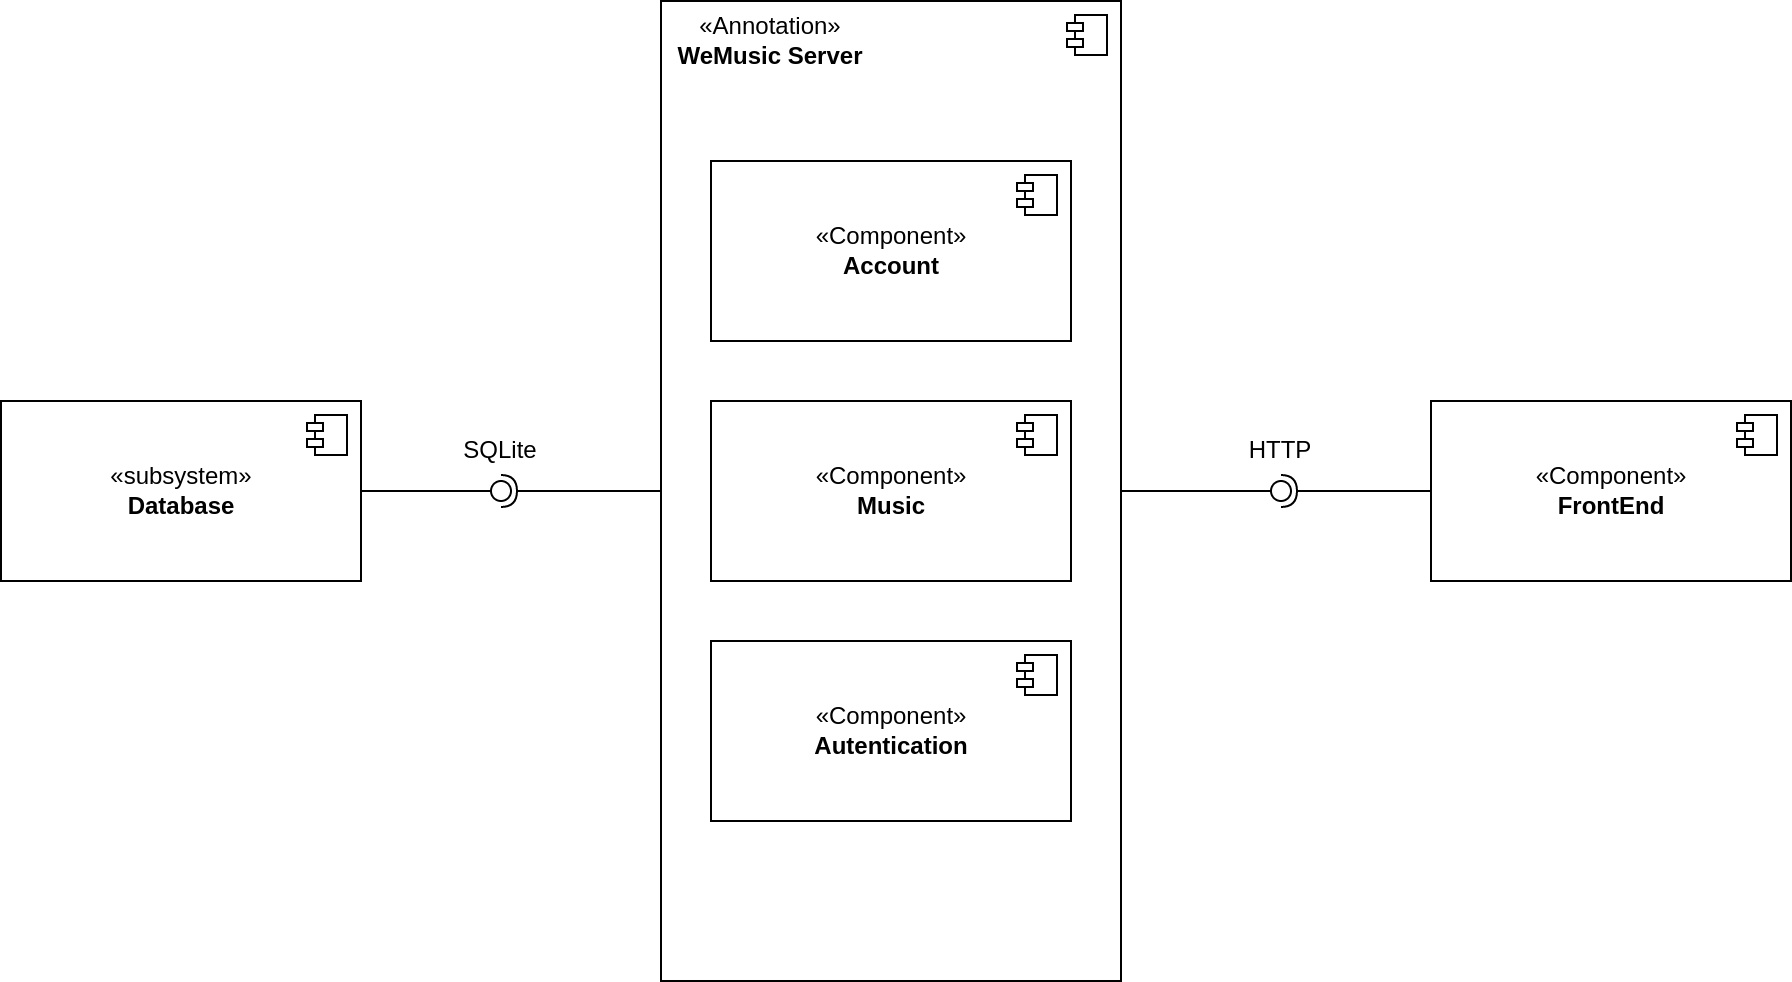
\includegraphics[scale=0.20]{component_diagram_v00.png}
    \caption{UML Component Diagram}
    \label{fig-uml-component-diag}
\end{figure}



\newpage
\section{UML Class Diagram}
Il Class Diagram in UML ha come obiettivo quello di descrivere il sistema 
visualizzando i diversi tipi di oggetti all'interno di esso e le relazioni 
statiche che esistono fra loro: sono descritte in maniera più approfondita 
le tre componenti già precedentemente analizzate, ovvero Account, Musica e 
Autenticazione.
In questo caso vengono rappresentati in unico diagramma il Data Class Diagram 
e l'interface/Package Diagram.
Il primo descrive le classi che compongono la struttura dell'applicazione 
delle entità presenti al suo interno; il secondo rappresenta il diagramma
 dei package che riassumono la struttura logica dell’applicazione 
e delle interfacce che verranno implementate nelle successive iterazioni.
Vengono anche illustrate le operazioni e gli attributi delle classi. 
\subsection{\textbf{Data Class Diagram}}

\begin{figure}[H]
    \centering
    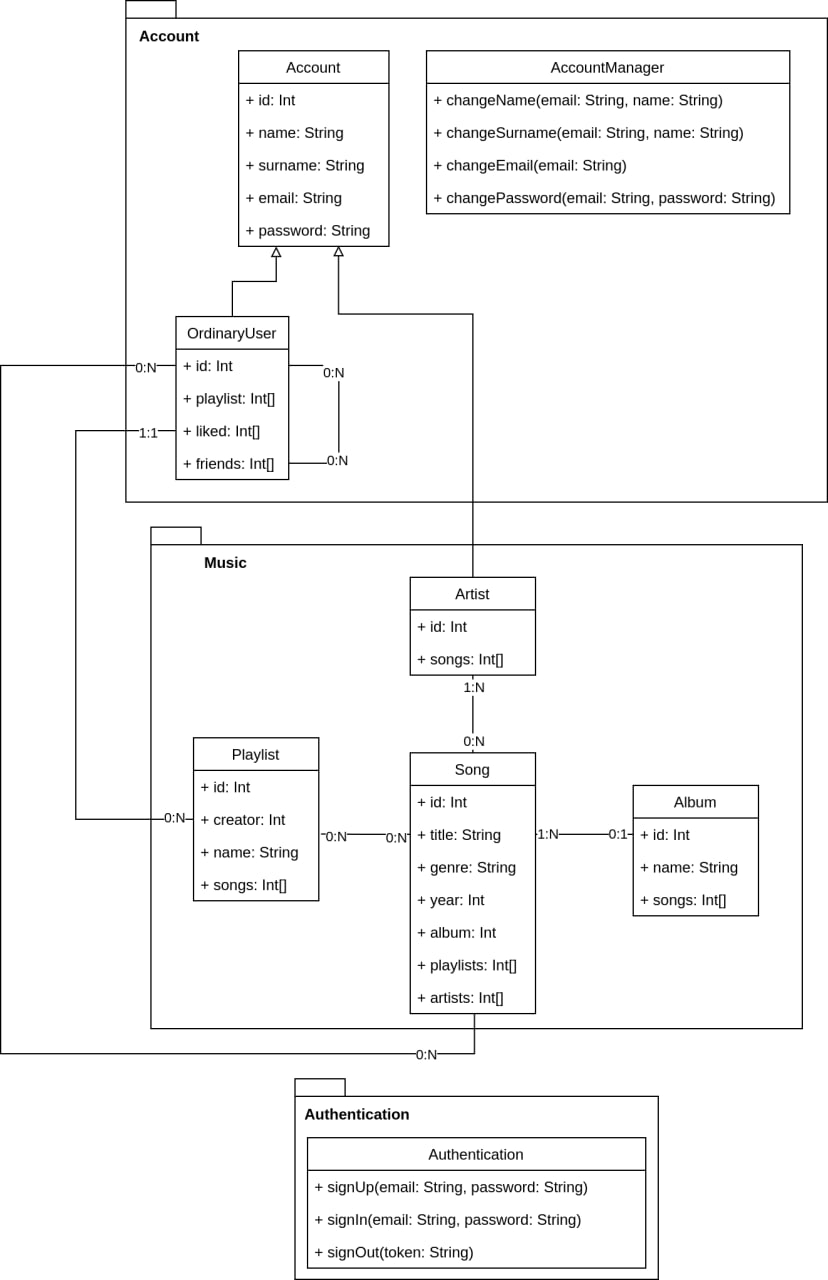
\includegraphics[scale=0.45]{class_diagram_v0.jpeg}
    \caption{UML Class Diagram}
    \label{fig-uml-class-diag}
\end{figure}



\subsection{\textbf{Interface and Package Class Diagram}}